%!TEX root = ../dissertation_vkslm.tex

\chapter{Experiments Result}

As described in Chapter \ref{ch:exp}, two different experiments are
carried out in order to analyze the quality of the synthetic
signatures and the feasibility of synthetically increasing the
enrollment set samples. The goal of the experiments is threefold, namely:
\begin{inlinelist}
  \item measure the similarity between real
  and synthetic images
  \item assess whether using synthetic
  signatures affects the recognition performance
  \item analyze the feasibility of using real and synthetic signatures
  on the enrollment set
\end{inlinelist}.

We compare our results with the state of the art, specifically the the approach proposed by Diaz \cite{diaz2014generation}. Our proposed method is compared with the ``Image enhanced'' synthetic signatures made available as part of the BiosecurID \cite{biosecurid} dataset. The reported EER is achieved for both approaches on the same experimental conditions.

\section{Experiment 1}
In order to evaluate the performance of the synthetic signature signatures described in Sect. II and the state of the art, two different protocols are followed: 
\begin{itemize}
\item mono-session: signatures from the first session on the enrollment set
\item multi-session: one signature per session.
\end{itemize}


\begin{table}[!htb]
%% increase table row spacing, adjust to taste
\renewcommand{\arraystretch}{1.3}
% if using array.sty, it might be a good idea to tweak the value of
% \extrarowheight as needed to properly center the text within the cells
\caption{EER for real, synthetic samples from Diaz \cite{diaz2014generation} and our proposed method synthetic off-line signatures, for all the approaches considered under the two possible scenarios (i.e., random and skilled forgeries)}
\label{exp1_results_table}
\centering
%% Some packages, such as MDW tools, offer better commands for making tables
%% than the plain LaTeX2e tabular which is used here.
\begin{tabular}{|l|l|l|l|}
	\hline
	\multicolumn{1}{|c|}{\multirow{2}{*}{\textbf{Mode}}} & \multicolumn{3}{c|}{\textbf{Skilled Forgeries}}          \\ \cline{2-4} 
	\multicolumn{1}{|c|}{}                               & \textbf{Real} & \textbf{Diaz} & \textbf{Proposed method} \\ \hline
	\textbf{mono-session}                                & 20.28\%            & 23.19\%            & 18.38\%                       \\ \hline
	\textbf{multi-session}                               & 17.59\%            & 22.27\%            & 16.48\%                       \\ \hline
	\multirow{2}{*}{}                                    & \multicolumn{3}{c|}{\textbf{Random Forgeries}}           \\ \cline{2-4} 
	& \textbf{Real} & \textbf{Diaz} & \textbf{Proposed method} \\ \hline
	\textbf{mono-session}                                & 9.07\%            & 10.65\%            & 9.99\%                       \\ \hline
	\textbf{multi-session}                               & 5.60\%            & 10.00\%            & 6.48\%                       \\ \hline
\end{tabular}

\end{table}

Table \ref{exp1_results_table} shows the EER achieved by the
real and the synthetic signatures databases. As it
may be observed, under the random forgeries scenario, the
EERs achieved by the real and both types of synthetic signatures
are very close. On the other hand we observe that under the skilled forgeries our proposed method synthetic signatures EERs yields better performance than both the real dataset and the synthetic signatures generated by Diaz.

In Figure \ref{exp1} (left - mono-session, right - multi-session) we
may observe that the behaviour of the system with real (gray dotted) and our proposed method synthetic signatures is quite similar, regardless of
the training protocol or the scenario considered. Nevertheless, our proposed method synthetic samples show a bigger discriminative power for skilled forgeries.

\begin{table}[!htb]
	%% increase table row spacing, adjust to taste
	\renewcommand{\arraystretch}{1.3}
	% if using array.sty, it might be a good idea to tweak the value of
	% \extrarowheight as needed to properly center the text within the cells
	\caption{EER for real, synthetic samples from Diaz \cite{diaz2014generation} and our proposed method synthetic off-line signatures for the Experiment 2 under the two possible scenarios, i.e., random (RF) and skilled forgeries (SF)}
	\label{exp2_results_table}
	\centering
	%% Some packages, such as MDW tools, offer better commands for making tables
	%% than the plain LaTeX2e tabular which is used here.
	\begin{tabular}{|l|l|l|}
		\hline
		\multicolumn{1}{|c|}{\textbf{Genuine Training}} & \multicolumn{1}{c|}{\textbf{SF}} & \textbf{RF} \\ \hline
		\textbf{4 real samples}                                         & 21.55\%                     & 10.26\%                         \\ \hline
		\textbf{4 real + 4 real samples}                       & 19.72\%                      & 7.63\%                        \\ \hline
		\textbf{4 real + 4 synthetic from Diaz}                           & 24.19\%                         & 7.72\%                \\ \hline
		\textbf{4 real + 4 synthetic from the Proposed Method}                           & 19.17\%         & 9.74\%                        \\ \hline
	\end{tabular}

\end{table}
\begin{figure}[!htb]
	\centering
	\label{exp2}
	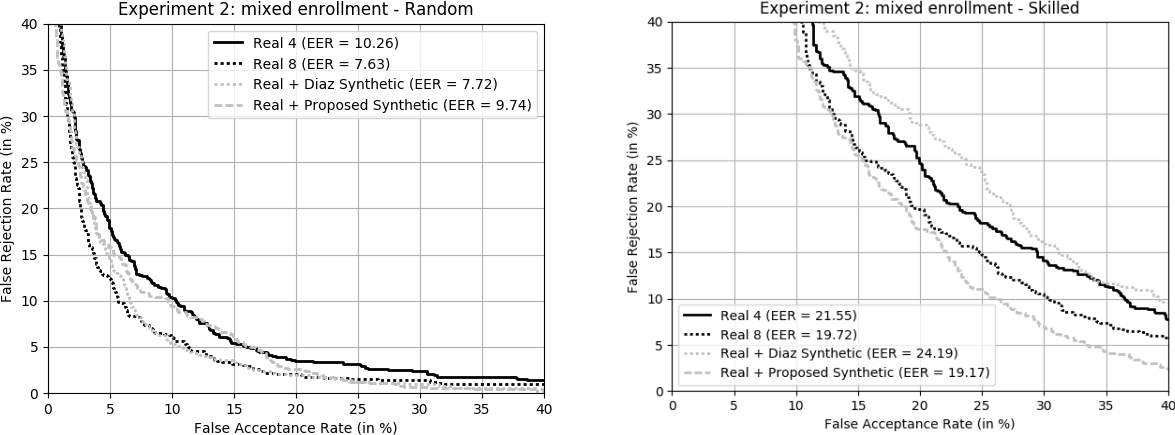
\includegraphics[width=5.0in]{rocs/experiment2}
	% where an .eps filename suffix will be assumed under latex, 
	% and a .pdf suffix will be assumed for pdflatex; or what has been declared
	% via \DeclareGraphicsExtensions.
	\caption{DET curves for real off-line signatures and synthetic signatures (from Diaz and our proposed method), for the second experiment, for the two scenarios considered (random and skilled impostors)}

\end{figure}
\section{Experiment 2}
In the last experiment, the feasibility of synthetically
increasing the enrollment set is analyzed. As described in
Sect. III, three different enrollment sets are considered. As it
may be observed in Figure \ref{exp2}, the DET curves for the
mixed enrollment (real + synthetic, grey dashed line), show a
better performance compared to the case with only four real
enrolled samples (black line), regardless of the operating point or the scenario considered. More specifically, the EER decreases from 10.26\% to 9.74\% on the random forgeries scenario and from 21.55\% to 19.17\% for skilled forgeries, respectively. The addition of synthetic samples for training thus leads to better recognition results.


It should also be noted that the behavior of the mixed enrollment is similar to the scenario with eight real enrolled samples (i.e., using eight real samples instead of
four real and four synthetic, black line) for skilled forgeries, and even yields a small improvement on the skilled forgery recognition rates. 

We may thus conclude that, our proposed system can be a good alternative to synthetically increase the off-line signatures samples when complementary on-line samples are available in order to increase the accuracy of the off-line verification system.